\documentclass[a4paper,utf8]{article}
\usepackage{graphicx}
\usepackage[heading,fancyhdr]{ctex}
\usepackage{amsmath,amssymb,geometry,ulem}
\usepackage{array,tabularx,tabulary,mhchem,xspace}
\usepackage{floatrow,subfig,multirow,bigstrut}
\usepackage{siunitx,booktabs,longtable,nameref}
\lineskiplimit=1pt
\lineskip=3pt
\geometry{
    top=25.4mm, 
    left=25mm, 
    right=25mm, 
    bottom=25mm,
    headsep=5.9mm,
}
\ctexset{
    chapter = {
        name = {实验,},
        beforeskip = {-23pt}
    }
}
\newcommand{\fgref}[1]{图~\ref{#1}\xspace}
\newcommand{\seqref}[1]{式~(\ref{#1})}
\newcommand{\expinfo}[6][无]{
    {\zihao{-3}\bfseries\songti
    实验名称:\uline{\hfill\mbox{#2}\hfill} \\[2.9mm]
    学\quad 号:\uline{\makebox[25mm]{#3}}\hfill
    姓\quad 名:\uline{\makebox[25mm]{#4}}\hfill
    班\quad 级:\uline{\makebox[25mm]{#5}} \\[2.9mm]
    合作者:\uline{\makebox[25mm]{#1}} \hfill
    桌\quad 号:\uline{\makebox[25mm]{}}\hfill\makebox[25mm+4em]{}\\[2.9mm]
    指导教师:\uline{\makebox[30mm]{#6}}\hfill\mbox{} \\[2.9mm]
    实验日期:\uline{\makebox[30mm]{}}\hfill\mbox{} \\[58.7mm]
    }
}%\expinfo[合作者]{实验名称}{学号}{姓名}{班级}{指导教师}
\newcommand{\pointingbox}{
    {\zihao{4}\bfseries\songti%
    实验考核\\[3mm]
    \extrarowheight=3mm
    \begin{tabularx}{150mm}{|X|X|X|X|X|}\hline
        \hfil 项目 \hfil  & \hfil 实验预习 \hfil & \hfil 实验过程 \hfil & \hfil 分析与讨论 \hfil & \hfil 总评 \hfil \\[3mm] \hline
        \hfil 评价 \hfil &  &  &  &  \\[3mm] \hline
    \end{tabularx}
    }
}
\newcommand{\derivative}[2]{\frac{\mathrm{d} #1}{\mathrm{d} #2}}
\newcommand{\thinking}[2]{\textbf{#1}\\
答:\begin{minipage}[t]{0.85\textwidth}
    #2
\end{minipage}}

\pagestyle{fancy}
\fancyhf{}
%\fancyhead[C]{材料科学基础实验}
%\fancyfoot[C]{\thepage}
\fancyhead[EC]{\leftmark} \fancyhead[OC]{\rightmark}
\fancyhead[EL,OR]{\thepage}
\fancypagestyle{plain}{\renewcommand{\headrulewidth}{0pt}\fancyhf{}}

\newcounter{Rownumber}
\newcommand*{\Rown}{\stepcounter{Rownumber}\theRownumber}
\newcounter{sample}
\newcommand*{\Sam}{\stepcounter{sample}\thesample}
\newcounter{Fignumber}
\newcommand*{\Fign}{\stepcounter{Fignumber}\theFignumber}

\newcommand*{\resetRown}{\setcounter{Rownumber}{0}}
\newcommand{\qrange}[3]{\qtyrange[range-phrase = \text{$\sim$},range-units =single]{#1}{#2}{#3}}
\floatsetup[table]{capposition=top}
\newcolumntype{C}{>{\hfil}X<{\hfil}}
\renewcommand{\Nameref}[1]{\textbf{\ref{#1}~\nameref{#1}}}
\newcommand{\TTR}[0]{\watt\per\m\per\K} %导入导言
\begin{document}
\begin{center}
    {\mbox{}\\[7em]\zihao{2}\bfseries\songti%
    材料科学基础实验预习报告}\\[34mm]
    \expinfo{金属材料力学、热学性能参数测量}{22301077}{张蕴东}{22高分子}{李继玲}
    {\zihao{4}\bfseries\songti
    实验考核\\[3mm]
    \extrarowheight=3mm
    \begin{tabularx}{150mm}{|X|X|X|X|X|}\hline
        \hfil 项目 \hfil  & \hfil 实验预习 \hfil & \hfil 实验过程 \hfil & \hfil 分析与讨论 \hfil & \hfil 总评 \hfil \\[3mm] \hline
        \hfil 评价 \hfil &  &  &  &  \\[3mm] \hline
    \end{tabularx}
    }
\end{center}
\newpage
\part{动态悬挂法测量金属材料杨氏模量}
\section{实验目的}
    \begin{itemize}
        \item 理解动力学振动法测量材料杨氏模量的基本原理;
        \item 熟悉示波器的使用,学会用示波器观察信号和识别共振; 
        \item 学会用外延法处理实验数据, 理解本实验采用外延法的原因。
    \end{itemize}
\section{实验原理}%简单描述,含必要的公式和附图;
    材料加工制备或者工程应用中都会受到外力作用,受力后材料会发生变形:外力较小时发生弹性变形,持续增加外力逐渐发生塑性变形甚至断裂。在这些变形中,弹性变形首先发生,是其他变形的先行阶段,同时在塑性变形中也会伴随着弹性变形。对于理想的弹性变形,在弹性限度内材料所受应力与其应变保持线性函数关系,满足胡克定律,即弹性限度内应力、应变比值为一确定常量,定义该常数为材料的杨氏模量,表征材料抵抗弹性形变的能力。杨氏模量是材料最具特征的力学性能参数,是材料在实际工程设计和机械设计中极为重要的参考量。\par
    典型而常用的拉伸法即为静态法测量材料的杨氏模量,但这种静态拉伸法仅适用于材料形变量大,延展性好的情况,对于脆性材料如玻璃、陶瓷等不适用。动态法适用材料范围广,可测量脆性材料,适用于不同的温度环境,测量结果稳定,理论同实验吻合度高。这些测量上的优越性使得动态法测量杨氏模量在实际应用中应用非常广泛,是国家标准指定的一种测量杨氏模量的方法。\par
    本实验即采用动态法测量不同金属试样的杨氏模量,具体方法为:将一根截面均匀的棒状试样通过悬线悬挂在两只传感器(一只激振,一只拾振)下面,试样端部不受其他外力,满足自由振动,由此对试样进行激振从而检测出其振动时的固有基频,而后可测得材料的杨氏模量。\par
    在一定条件下,对于具有确定材料组成和确定形状的待测试样,其固有频率的大小既与待测试样自身的几何形状、尺寸和质量有关,还与组成试样的材料本身的杨氏模量直接相关。因此,如果我们通过实验测得某试样在一定温度下的固有频率,就可以通过简单的几何尺寸和质量的测量算得组成试样的材料在此温度下的杨氏模量。由此,基于此方法对材料杨氏模量的测量关键问题在于如何准确得测量试样本身的固有频率。\par
    对试样棒建模可得到原始方程:
    \begin{equation}
        \frac{\partial^4y}{\partial^4x}=\frac{\rho S}{EJ}\cdot\frac{\partial^2y}{\partial t^2}
    \end{equation}
    式中 $\rho,S,E,J$ 分别表示试样的材料密度、试样棒的截面积、试样材料的杨氏模量和试样棒某一截面的惯量矩($J=\int y^2ds$)。\par
    最后我们得到,圆柱形棒材的杨氏模量 E 可以表示为:
    \begin{equation}
        E=1.6067\frac{l^3m}{d^4}f^2\label{eq:2}
    \end{equation}
    式中 $l$ 为棒长、 $d$ 为圆形棒的截面直径,单位 \unit{\m} ;$m$ 为棒的质量,单位 \unit{\kg} ; $f$为试样固有频率,单位 \unit{\Hz}。 所以,如果实验中测定了试样在不同温度时的固有频率 $f$,即可通过上式计算出试样在对应温度下的杨氏模量 $E$。在 SI 中杨氏模量的单位为\unit{\N\per\m^2}。\par
    微分方程的解还说明了:试样作基频振动时,存在距离端面分别为 $0.224l$ 和$0.776l$的两个节点。显然,节点处是不振动的,阻尼为零,此时无阻尼自由振动的振动频率就是试样的固有频率,即当支撑点为节点时,测得的共振频率就是试样的固有频率。但是,因为节点处不振动无法实现激振,故而实验时悬丝不能吊挂在试样节点上而只能挂在节点附近。在实际测量中,悬丝和悬挂点均会对试样的自由振动产生阻尼,因而,所检测到的共振频率会随着悬挂点位置的不同而变化,且悬挂点偏离节点越远,可检测的信号越强,但共振频率将偏离固有频率越大。所以,要测量振动试样的固有频率(基频频率),需要通过适当的数据处理获得试棒悬挂点为节点处时,试棒做无阻尼自由振动的基频频率。 
\section{实验仪器}%规格及参数
    DY-A型金属动态杨氏模量测定仪、金属动态杨氏模量测试台、待测金属试样、游标卡尺、螺旋测微计、天平、示波器等。 \par
    动态杨氏模量测量仪作为信号发生器输出等幅正弦波电信号,信号经放大器放大,通过悬线上方的激振传感器将电信号转变为机械振动,由悬线把机械振动传递给待测试样,待测试样因受到悬线作用的横向作用力而产生横振动。试样的横振动通过另一端的悬线传递给拾振传感器,通过拾振传感器将试样横振动转变为周期电信号,经放大器放大后输入示波器。当信号发生器的输出频率不等于此悬挂状态下试样的固有频率时,试样不发生共振,示波器上几乎没有信号波形显示或波形很小;当信号发生器的输出频率几乎接近试样相应悬挂状态下的固有频率时,试样发生共振,这时,示波器上波形会突然增大,此时信号发生器的输出信号频率,即为此时的共振频率,也是试样在此悬挂点悬挂时的固有频率。
\section{实验过程}%简述主要过程和实验内容
    \begin{enumerate}
        \item 首先测量出待测试样的长度 $l$,直径 $d$ 和质量 $m$ ,测量用具分别为游标卡尺、螺旋测微器和电子天平;
        \item 根据 \eqref{eq:2} 估算待测试样的固有频率。已知室温下待测试样不锈钢棒材和铜棒材的杨氏模量标准值分别为 \SI{2E+11}{\N\per\m^2} 和 \SI{1.2E+11}{\N\per\m^2},先估算试样的固有频率f,以便寻找共振点。
        \item 要使试样共振频率为待测试样的固有频率,试样本身须作无阻尼自由振动,要求在操作中,悬挂点须在两个节点位置(距离端面分别为 $0.224l$ 和 $0.776l$ 处)。但实际上,悬挂点在节点处时因节点处 $y=0$ 无法实现试样激发振动。因此,在实际操作中,实际的吊扎位置要偏离节点;
        \item 在偏离节点且距离试样两端面等距离处选择两位置,记录两点位置x并作为悬挂点在此两位置处悬挂待测试棒。室温下测量该悬挂位置待测金属棒的共振频率f;试样共振状态的建立需要有一个过程,且共振峰十分尖锐。因此共振点附近调节信号频率时,必须十分缓慢的进行
        \item 在节点的两侧分别选择不同位置对待测试棒进行悬挂,之后按照4相同的方法,测出待测金属棒在不同悬挂点悬挂时的共振频率。要求节点两侧待测量悬挂位分别两个及以上;
        \item 以悬挂点$\frac{x}{l}$为横坐标,上述4和5测得的共振频率 $f$ 为纵坐标做图,可得悬挂点位置和共振频率之间的变化曲线。根据曲线变化规律,采用内插法或外延法处理实验数据,当 $x$ 逼近 $0.224l$ 时即可得到悬挂点在节点处的共振频率,根据前述基本原理,此时的共振频率为试样无阻尼自由振动的基频,亦即试样的固有频率;代入 \eqref{eq:2} 求得试样杨氏模量,与标准比对分析和讨论实验误差。 
    \end{enumerate}
\section{实验数据}
    \begin{table}[!ht]
        \centering\begin{tabular}{c c c c}\hline
            种类 & 直径 $\bar{d}$ & 长度 $\bar{L}$ & 质量 $\bar{m}$\\ \hline
            不锈钢棒 & \SI{6.00}{\mm} & \SI{150.16}{\mm} & \SI{33.279}{\g} \\ 
            铜棒 & \SI{6.00}{\mm} & \SI{150.00}{\mm} & \SI{35.379}{\g} \\ \hline
        \end{tabular}
    \end{table}\par
    \begin{table}[!ht]
        \caption{不锈钢棒悬挂不同位置得到的频率}
        \centering\begin{tabular}{c c c c c c}\hline
            次数 & 1 & 2 & 3 & 4 & 5\\ \hline
            距离 (mm) & 10.0 & 20.0 & 25.0 & 40.0 & 45.0 \\ 
            共振频率 (Hz) & 1179.0 & 1174.8 & 1172.4 & 1174.8 & 1176.0\\ \hline
        \end{tabular}
    \end{table}\par
    如图,用四阶多项式拟合得到:$ y =  1163.14286 + 3.69029 * x  -0.2788 * x^2 + 0.0075 * x^3 - \num{6.62857E-5} *x^4 $ \par
    \begin{figure}[!ht]
        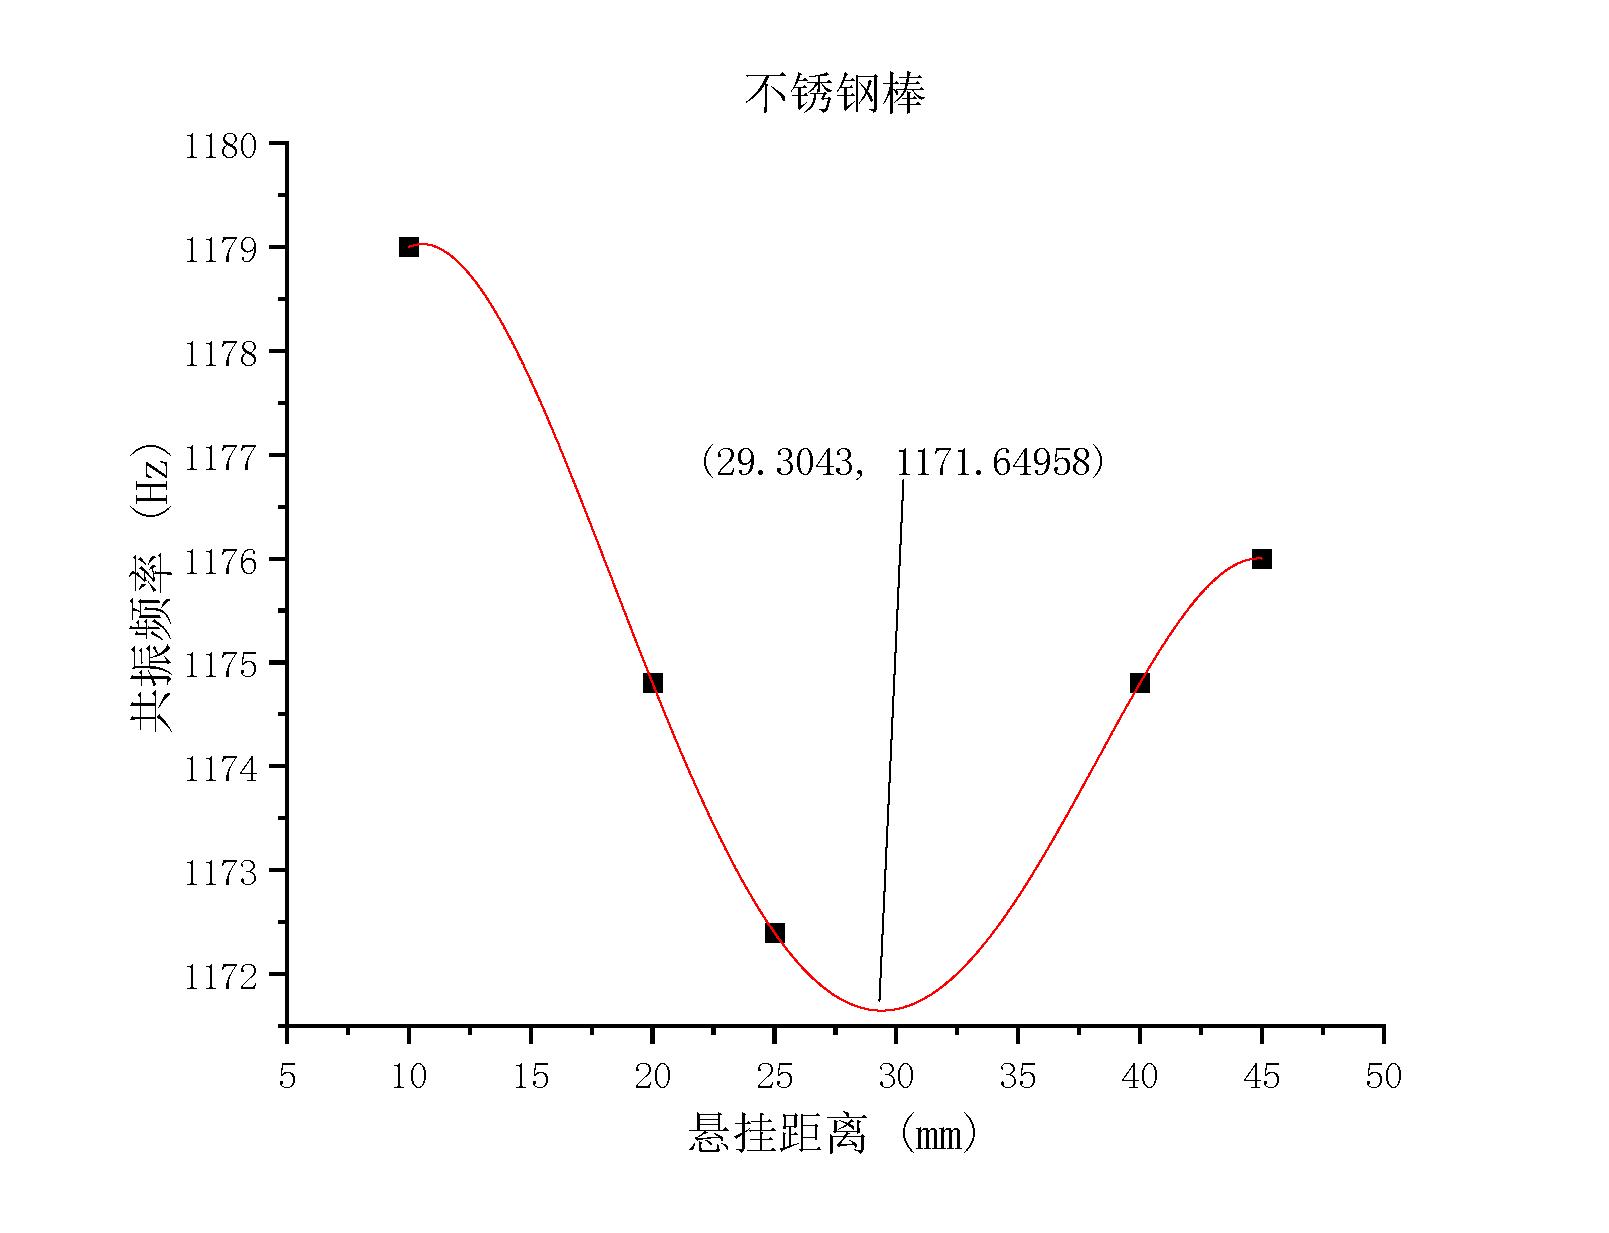
\includegraphics[width=0.6\textwidth]{fig1.pdf}
    \end{figure}\par
    计算得到不锈钢棒的杨氏模量为:$E_1=1.9176*10^{11}$ , $\text{相对误差:} 4.11 \%$
    \begin{table}[!ht]
        \caption{铜棒悬挂不同位置得到的频率}
        \centering\begin{tabular}{c c c c c c}\hline
            次数 & 1 & 2 & 3 & 4 & 5\\ \hline
            距离 (mm) & 10.0 & 20.0 & 25.0 & 40.0 & 45.0 \\ 
            共振频率 (Hz) & 846.0 & 842.1 & 836.8 & 840.8 & 841.7 \\ \hline
        \end{tabular}
    \end{table}\par
    如图,用四阶多项式拟合得到:$ y =  785.17143 + 12.48348 * x  -0.83557 * x^2 + 0.02142 * x^3 - \num{1.86476E-4} * x^4 $ \par
    \begin{figure}[!ht]
        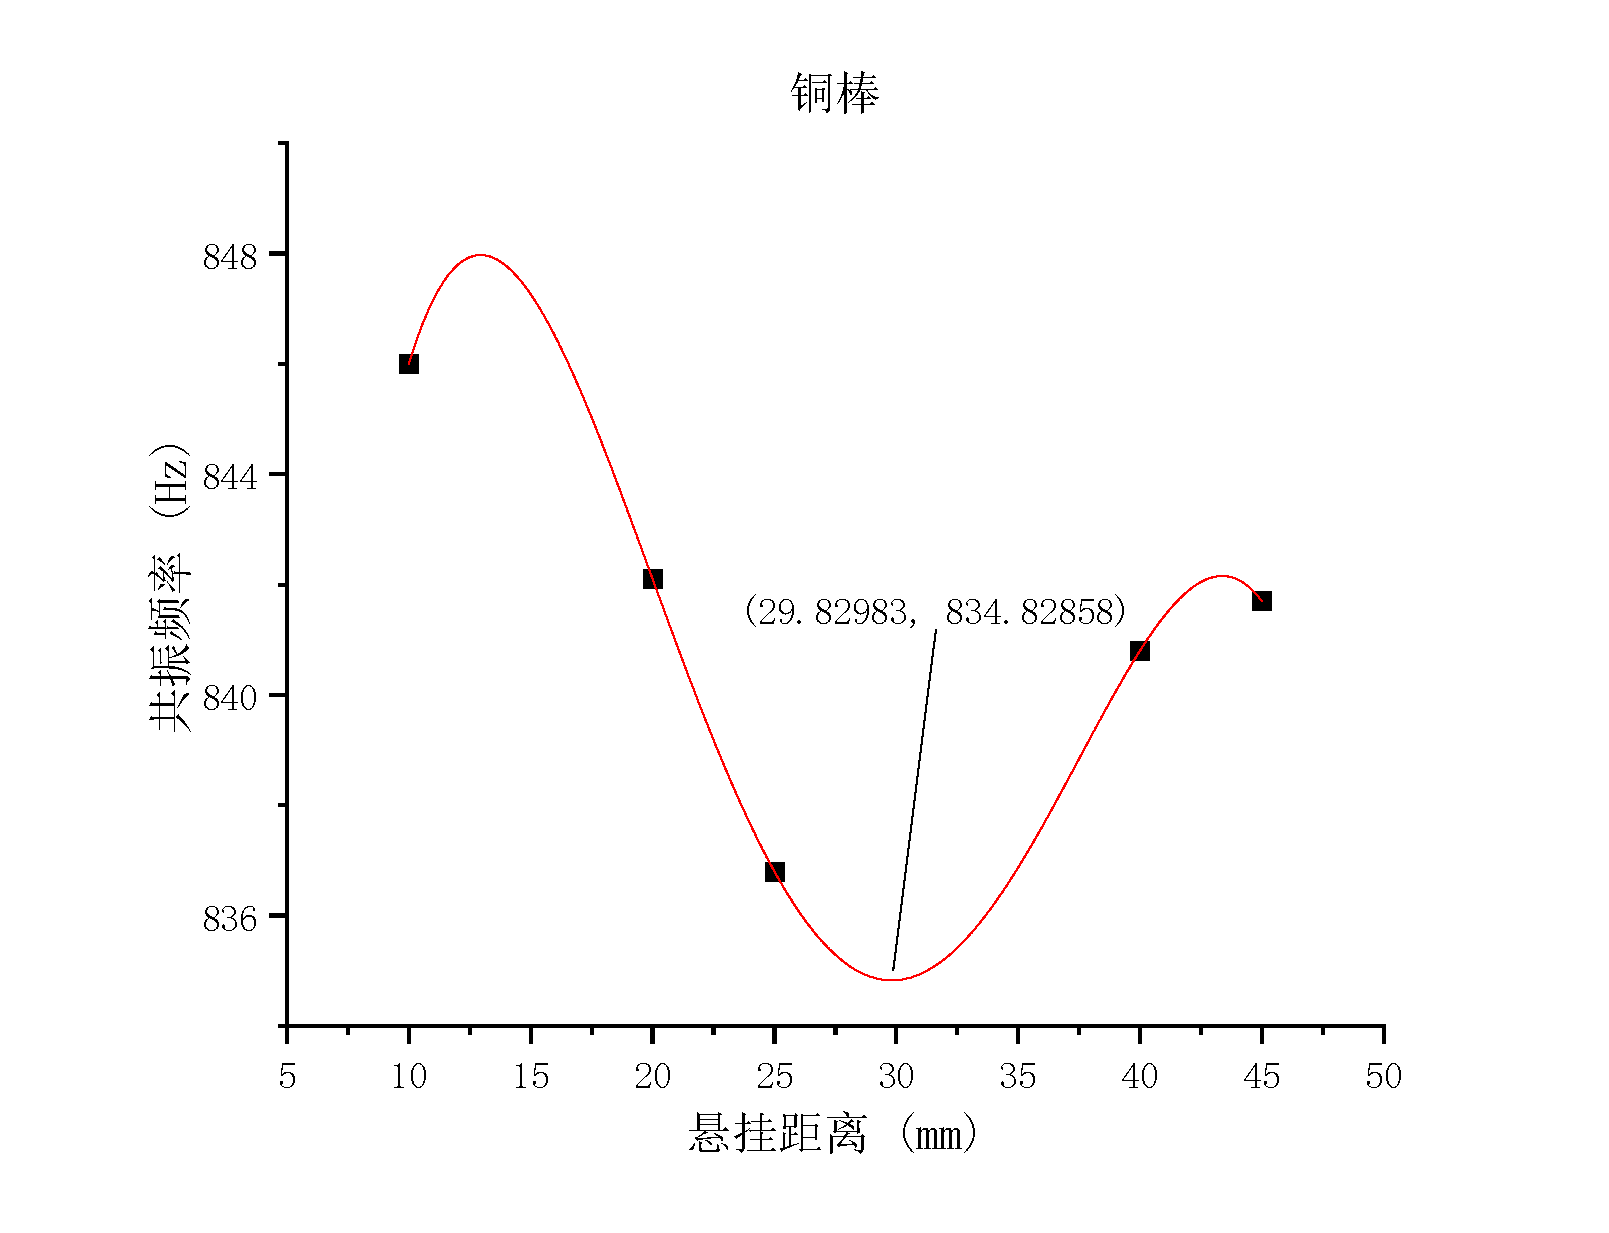
\includegraphics[width=0.6\textwidth]{fig2.pdf}
    \end{figure}\par
    计算得到铜棒的杨氏模量为:$E_2=1.03166*10^{11}$ , $\text{相对误差:} 14.03 \%$\newpage
    本次实验测得的数据虽然与真实值有所偏差,但是考虑到在动态悬挂时测得的点有限,拟合无法很好反映真实情况、测量时的误差、装置频率变化大,种种原因都会导致计算结果出现偏差。此外,试样也本身并非标准的样品,测得的杨氏模量应当与标准值有所偏差,这些都是正常情况,
\section{思考题}
    \subsection{什么是杨氏模量?杨氏模量的意义?} 
    杨氏模量是材料力学中的一个重要参数,指在材料受到拉伸或压缩时,单位面积内的应力与相应的应变之间的比值,通常用符号 $E$ 表示。换言之,杨氏模量衡量了材料在受力时的刚度,即材料对外部应力的响应程度。其意义在于能够量化的比较材料的不同应力条件下的性能,更精确的指导工程设计。
    \subsection{试讨论,试样的长度 l、直径 d、质量 m、共振频率 f 分别应该采用什么规格
    的仪器测量?为什么?} 
    \begin{enumerate}
        \item $l,d$ 可以使用游标卡尺测量,以减小测量误差
        \item $m$ 可以使用分析天平称量,以减小测量误差
        \item $f$ 可以使用采样率高、带宽高、分辨率高的示波器采集、用分辨率更高的交流源来找到共振频率,以减小测量误差
    \end{enumerate}
\newpage
\part{基于迈克尔逊干涉测量金属材料线膨胀系数}
\setcounter{section}{0}
\section{实验目的}
    \begin{itemize}
        \item 观察材料的线膨胀现象,了解测量材料线膨胀系数的基本原理;
        \item 了解光学干涉现象及迈克尔逊干涉的基本原理及调节方法; 
        \item 理解测量微小尺寸变化的方法。
    \end{itemize}
\section{实验原理}%简单描述,含必要的公式和附图;
    由于微观粒子热运动的存在,绝大多数材料宏观上存在“热胀冷缩”现象,即物体存在受热时会膨胀,受冷时会收缩的特性。这种随温度变化而产生宏观尺寸变化的特性在材料的实际应用中应予以充分考虑,否则将产生不利影响,如因“热胀冷缩”可能会引起工程结构的损坏、仪表失灵等。线膨胀系数为了表征物体随温度变化其长度变化程度而引入的物理量,可定量分析材料热膨胀问题,是衡量材料热稳定性的重要指标。目前,对微小长度和其变化量的测量方法按照基本原理可分为三类:利用杠杆原理、利用光学干涉原理和利用螺旋测微原理直接测量。在几种测量方法中,利用光学干涉现象测量微小尺寸的结果精度最高,本实验即基于迈克尔逊干涉现象测量金属材料随温度变化在确定方向的伸长量,从而可得其线膨胀系数。\par
    线膨胀系数在数值上定义为固体材料每升高 \SI{1}{\degreeCelsius} 时单位长度的伸长量。对于同一材料,在不同的温度区间,线膨胀系数是不同的,但在温度变化不太大的情况下,通常认为材料的线膨胀系数可近似为常量。假设在确定的温度范围内,一固态物体在确定方向上温度为 $t-0$(单位:\unit{\degreeCelsius})时长度为 $L_0$,对物体进行升温,当温度为 $T$ 时,其长度为 $L$,伸长量 $\varDelta L=L-L0$。实验表明,物体在确定方向上的单位伸长量与温度增量$\varDelta T$近似成正比,即:
    \begin{equation}
        \frac{\varDelta L}{L_0} = \alpha \times \varDelta T \Longrightarrow  \alpha=\frac{\varDelta L}{L_0 \varDelta T}
    \end{equation}
    $\alpha$ 即为该物体在此温度区间内的线膨胀系数,表征了组成材料在此确定方向上的受热膨胀(或收缩)的程度。温度变化不大时,材料的线膨胀系数 $\alpha$ 可近似为常数。\par
    本实验基于迈克尔逊干涉实验测量线膨胀系数,具体方法为:将待测金属试样置于左下侧温控炉内并通过温控炉在一定温度范围内改变待测试样温度,试样将受热发生膨胀而伸长,推动反射镜向上移动,从而使迈克尔逊干涉中其中的一路的光程发生变化,因而,两路光线的光程差改变,由此可实现干涉条纹的动态观察。\par
    经推导得到本次实验计算用公式:
    \begin{equation}
        \alpha=\frac{N\frac\lambda2}{L_1(t_2-t_1)}
    \end{equation}
\section{实验仪器}%规格及参数
    热膨胀实验仪
\section{实验过程}%简述主要过程和实验内容
    \begin{enumerate}
        \item 准备待测试样,将待测试样放入温控炉中;
        \item 根据迈克尔逊干涉光路原理调节光路,观察干涉条纹
        \item 测量和读取数据
        \item 根据所测数据,计算待测试样的线膨胀系数
        \item 本次实验要求测量黄铜和硬铝两个试样并对测量数据做表记录         
    \end{enumerate}
\section{实验数据}
    \begin{table}[!ht]
        \centering
        \begin{tabular}{|c|c|c|c|}
        \hline
            试样 & $\bar{L_0}$ & $\bar{\Delta t}$ & N \\ \hline
            铜棒 & 150.00 & 0.98 & 10 \\ 
            铝棒 & 149.99 & 0.80 & 10 \\ \hline
        \end{tabular}
    \end{table}
    计算得到试样的线膨胀系数:
    \begin{align*}
        \alpha_1 & =\frac{N\frac\lambda2}{L_0 {\Delta t}_1}=\num{2.0952e5}~\unit{\per\degreeCelsius}\\
        \alpha_2 & =\frac{N\frac\lambda2}{L_0 {\Delta t}_1}=\num{2.4368e5}~\unit{\per\degreeCelsius}\\
    \end{align*}
    相对误差分别为:$0.73 \%,3.25\%$,可以发现本实验的测量结果与事实吻合较好,体现了实验操作的准确与严谨,也反映出该实验的方案与器材合理、测量误差小。误差分析见思考题。
\section{思考题}
    \subsection{测量材料线膨胀系数的意义并举例说明} 
    线膨胀系数是描述材料在温度变化下尺寸变化的参数,通常用于工程设计和材料选择中。例如高铁轨道由于工作状况变化跨度大,长轨道在温度变化下的长度变化将非常明显,此时就可以通过钢材的线膨胀系数来评估其适不适合用来铺设钢轨。
    \subsection{分析实验中影响实验结果的因素有哪些?} 
    \begin{enumerate}
        \item 实验当天的温度、湿度所带来的误差。仪器本身精度的影响,如温控仪本身只能取到小数点后一位,会产生一定的误差。观察干涉条纹时难以判断何时是刚刚好出现一个干涉环,时间测量上也有误差。
        \item 光源的频率或强度的微小变化可能导致测量误差
        \item 迈克尔逊干涉仪的光路必须保持稳定,以确保干涉条纹的清晰度和稳定性,正规的光学实验常使用气动缓冲来保证平台的水平。
    \end{enumerate}
\end{document}